\documentclass[border=5pt]{standalone}
\usepackage{tikz}
\usetikzlibrary{decorations.pathreplacing}
\usepackage{xcolor}

\definecolor{Garnet}{HTML}{73000A}
\definecolor{NinetyBlack}{HTML}{363636}
\definecolor{SeventyBlack}{HTML}{5C5C5C}
\definecolor{FiftyBlack}{HTML}{A2A2A2}
\definecolor{ThirtyBlack}{HTML}{C7C7C7}
\definecolor{Atlantic}{HTML}{466A9F}

\tikzset{every node/.append style={rounded corners=0pt}}

\begin{document}
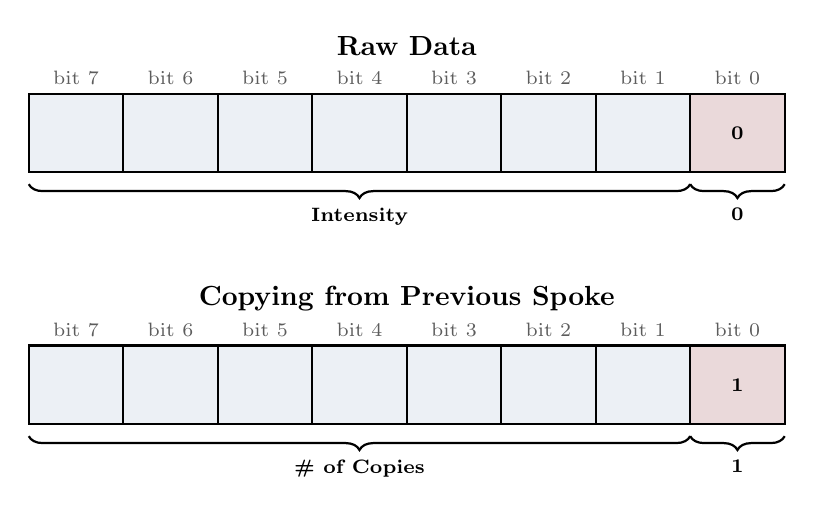
\begin{tikzpicture}

% ── Literal ──
\node[font=\normalsize\bfseries] at (4.8, 4.6) {Raw Data};

\foreach \i/\v in {0/7, 1/6, 2/5, 3/4, 4/3, 5/2, 6/1, 7/0} {
    \node[font=\scriptsize, color=SeventyBlack] at (0.6 + \i*1.2, 4.2) {bit \v};
}

% 8 cells
\foreach \i in {0,...,7} {
    \draw[thick] (0 + \i*1.2, 3.0) rectangle (1.2 + \i*1.2, 4.0);
}

% Amplitude fill — bits 7:1
\fill[Atlantic!10] (0, 3.0) rectangle (8.4, 4.0);
\foreach \i in {0,...,6} {
    \draw[thick] (0 + \i*1.2, 3.0) rectangle (1.2 + \i*1.2, 4.0);
}

% Flag fill — bit 0
\fill[Garnet!15] (8.4, 3.0) rectangle (9.6, 4.0);
\draw[thick] (8.4, 3.0) rectangle (9.6, 4.0);
\node[font=\scriptsize\bfseries] at (9.0, 3.5) {0};

% Braces below
\draw[decorate, decoration={brace, amplitude=5pt, mirror}, thick]
    (0, 2.85) -- (8.4, 2.85) node[midway, below=5pt, font=\scriptsize\bfseries] {Intensity};
\draw[decorate, decoration={brace, amplitude=5pt, mirror}, thick]
    (8.4, 2.85) -- (9.6, 2.85) node[midway, below=5pt, font=\scriptsize\bfseries] {0};


% ── Repeat ──
\node[font=\normalsize\bfseries] at (4.8, 1.4) {Copying from Previous Spoke};

\foreach \i/\v in {0/7, 1/6, 2/5, 3/4, 4/3, 5/2, 6/1, 7/0} {
    \node[font=\scriptsize, color=SeventyBlack] at (0.6 + \i*1.2, 1.0) {bit \v};
}

% 8 cells
\foreach \i in {0,...,7} {
    \draw[thick] (0 + \i*1.2, -0.2) rectangle (1.2 + \i*1.2, 0.8);
}

% Count fill — bits 7:1
\fill[Atlantic!10] (0, -0.2) rectangle (8.4, 0.8);
\foreach \i in {0,...,6} {
    \draw[thick] (0 + \i*1.2, -0.2) rectangle (1.2 + \i*1.2, 0.8);
}

% Flag fill — bit 0
\fill[Garnet!15] (8.4, -0.2) rectangle (9.6, 0.8);
\draw[thick] (8.4, -0.2) rectangle (9.6, 0.8);
\node[font=\scriptsize\bfseries] at (9.0, 0.3) {1};

% Braces below
\draw[decorate, decoration={brace, amplitude=5pt, mirror}, thick]
    (0, -0.35) -- (8.4, -0.35) node[midway, below=5pt, font=\scriptsize\bfseries] {\# of Copies};
\draw[decorate, decoration={brace, amplitude=5pt, mirror}, thick]
    (8.4, -0.35) -- (9.6, -0.35) node[midway, below=5pt, font=\scriptsize\bfseries] {1};

\end{tikzpicture}
\end{document}
